%=======================================================================
%  CS-3810 Design Practices in Computer Science -- Assignment 2
%  Project 3: Interactive Data Structure and Algorithms Visualizer
%  Team PY -- Papaa Dennis Morindat, Yididiya Megenta
%
%  Technical design document. Sections 3-6 answer the Assignment 2 brief
%  directly. Design decisions made by the team are marked [A]; requirements
%  stated or directly implied by the project description are marked [R].
%
%  Compile with:  tectonic -X compile A2_PY.tex
%  Submission:    rename the compiled PDF to  A2_PY.pdf
%=======================================================================
\documentclass[11pt,a4paper]{article}

\usepackage[T1]{fontenc}
\usepackage{lmodern}
\usepackage[margin=2.3cm,top=2.7cm,bottom=2.7cm,headheight=14pt]{geometry}
\usepackage{amsmath,amssymb}
\usepackage{booktabs}
\usepackage{longtable}
\usepackage{array}
\usepackage{enumitem}
\usepackage{xcolor}
\usepackage{tikz}
\usetikzlibrary{arrows.meta,positioning,fit,backgrounds,calc,shapes.geometric}
\usepackage{listings}
\usepackage{caption}
\usepackage{float}          % [H]: pin floats exactly where they are written
\usepackage{fancyhdr}
\usepackage{microtype}
\usepackage{parskip}
\usepackage[hidelinks]{hyperref}

\setcounter{secnumdepth}{3}
\setcounter{tocdepth}{2}
\setlength{\emergencystretch}{2em}

%------------------------- colours -------------------------
\definecolor{reqc}{RGB}{0,102,51}
\definecolor{asmc}{RGB}{176,88,0}
\definecolor{primary}{RGB}{11,79,158}
\definecolor{boxc}{RGB}{235,242,250}
\definecolor{statec}{RGB}{232,240,254}
\definecolor{rulec}{RGB}{120,120,120}
\definecolor{codec}{RGB}{245,245,247}

%------------------------- column types -------------------------
\newcolumntype{L}[1]{>{\raggedright\arraybackslash}p{#1}}
\newcolumntype{C}[1]{>{\centering\arraybackslash}p{#1}}

%------------------------- shorthands -------------------------
\newcommand{\R}{\textcolor{reqc}{\textbf{[R]}}}     % stated requirement
\newcommand{\A}{\textcolor{asmc}{\textbf{[A]}}}     % team assumption / decision
\newcommand{\ct}[1]{\texttt{#1}}
\newcommand{\bigO}[1]{\ensuremath{\mathcal{O}(#1)}}
\newcommand{\norm}[1]{\ensuremath{\lvert #1 \rvert}}

%------------------------- code listings -------------------------
\lstdefinestyle{base}{
  basicstyle=\ttfamily\footnotesize,
  columns=fullflexible,
  keepspaces=true,
  breaklines=true,
  breakatwhitespace=false,
  showstringspaces=false,
  frame=single,
  framesep=5pt,
  rulecolor=\color{rulec},
  backgroundcolor=\color{codec},
  xleftmargin=8pt,
  xrightmargin=4pt,
  aboveskip=8pt,
  belowskip=8pt
}
\lstset{style=base}
% Pin every captioned listing exactly where it is written (requires the float package),
% so a listing can never drift past the subsection or table that follows it.
\lstset{floatplacement=H}
\lstdefinestyle{pseudo}{style=base,numbers=left,numberstyle=\tiny\color{rulec},numbersep=6pt}
\lstdefinestyle{ts}{style=base,numbers=none}
\lstdefinestyle{c}{style=base,numbers=left,numberstyle=\tiny\color{rulec},numbersep=6pt,
  language=C,keywordstyle=\color{primary}\bfseries,
  commentstyle=\color{rulec}\itshape,stringstyle=\color{asmc}}

\captionsetup{font=small,labelfont=bf,skip=6pt}
\renewcommand{\arraystretch}{1.12}

%------------------------- tikz styles -------------------------
\tikzset{
  comp/.style={draw=rulec, rounded corners=2pt, fill=boxc, align=center,
               inner sep=5pt, font=\small, text width=3.6cm, minimum height=1.35cm},
  layer/.style={draw=rulec, rounded corners=2pt, fill=boxc, align=left,
                inner sep=6pt, font=\small, text width=14.2cm},
  auxbox/.style={draw=rulec, rounded corners=2pt, fill=statec, align=center,
                 inner sep=4pt, font=\footnotesize},
  e/.style={-{Stealth[length=2.2mm]}, draw=rulec, thick},
  ed/.style={-{Stealth[length=2.2mm]}, draw=rulec!70, dashed},
  ebi/.style={{Stealth[length=2.2mm]}-{Stealth[length=2.2mm]}, draw=rulec},
  lbl/.style={font=\scriptsize, inner sep=1.6pt, fill=white}
}

%------------------------- headers -------------------------
\pagestyle{fancy}
\fancyhf{}
\fancyhead[L]{\footnotesize CS-3810: Design Practices in Computer Science}
\fancyhead[R]{\footnotesize Assignment 2: Technical Design}
\fancyfoot[C]{\footnotesize\thepage}
\renewcommand{\headrulewidth}{0.3pt}

\begin{document}

%=======================================================================
\begin{center}
  {\large\bfseries Department of Computer Science}\\[2pt]
  {\small Ashoka University}\\[10pt]
  {\LARGE\bfseries CS-3810: Design Practices in Computer Science}\\[6pt]
  {\large\bfseries Assignment 2: Technical Design}\\[10pt]
  {\large\bfseries Project 3: Interactive Data Structure and Algorithms Visualizer}
\end{center}

\vspace{2pt}
\begin{center}
\renewcommand{\arraystretch}{1.25}
\begin{tabular}{@{}L{4.2cm}L{10.4cm}@{}}
\toprule
\textbf{Assignment Type} & Group Assignment \\
\textbf{Marks} & 100 \\
\textbf{Submission Format} & PDF generated from \LaTeX \\
\textbf{Submission} & Google Classroom \\
\textbf{Naming Convention} & A2\_PY.pdf \\
\bottomrule
\end{tabular}
\end{center}

%-----------------------------------------------------------------------
\section*{Document Status and Reading Guide}
\addcontentsline{toc}{section}{Document Status and Reading Guide}

\noindent\fcolorbox{rulec}{boxc}{%
\begin{minipage}{\dimexpr\linewidth-2\fboxsep-2\fboxrule\relax}
\textbf{Status.} This document is the second design-stage deliverable. It converts the
specification and requirements analysis of Assignment 1 into an implementable technical
design: the algorithms (Section~3), the data structures (Section~4), the software
architecture (Section~5) and the technology stack (Section~6). Together these four sections
answer every item of the Assignment~2 brief directly.
\end{minipage}}

\medskip
\textbf{Conventions.} Instruction~6 of the brief requires design decisions to be separated
from stated requirements. We keep the convention of Assignment~1:

\begin{itemize}[leftmargin=1.5em,topsep=2pt,itemsep=1pt]
  \item \R\ --- a requirement stated or directly implied by the project description.
  \item \A\ --- an assumption, design decision or extension made by our team.
\end{itemize}

\noindent\textbf{What this document adds to Assignment 1.} Assignment~1 fixed \emph{what}
the system must do. Assignment~2 fixes \emph{how} it will be built. The three load-bearing
decisions inherited from Assignment~1 and carried through every section here are: the
algorithm emits an immutable step trace rather than animating a live object; the interface
is a pure function of \ct{(trace, index)}; and the algorithm layer has no dependency on the
presentation layer.

\medskip
\noindent\textbf{Scope change since Assignment~1 (structures).} \A\ The graded structure set for
this iteration is

\begin{center}
\textbf{Linked List \quad Stack \quad Priority Queue \quad Tree (BST) \quad Graph.}
\end{center}

\noindent The Priority Queue is treated as a first-class visualised structure, implemented as a
binary min-heap and shown simultaneously as an array and as a complete binary tree. FIFO
queueing has not disappeared from the system: it remains the frontier container used by
breadth-first search in Section~3.5 and by level-order traversal in Section~3.4, and it is
rendered by the same auxiliary panel. Section~4.6 documents the queue as a \emph{supporting}
structure rather than a catalogue entry, and notes the single-catalogue-entry change that
would promote it back to a first-class structure if the brief requires it.

\medskip
\noindent\textbf{Reading path for a grader.} Section~3 (algorithms) $\to$ Section~4 (data
structures) $\to$ Section~5 (architecture, beginning with the diagram in Section~5.1) $\to$
Section~6 (technology stack).

%=======================================================================
\section{Purpose of the Assignment}

This document is the technical design for the Interactive Data Structure and Algorithms
Visualizer (Project~3). It follows the second design-stage brief, whose objective is to
translate the project specification and technical analysis from Assignment~1 into a concrete
technical design for implementation. Following the brief, it establishes:

\begin{itemize}[leftmargin=1.4em,topsep=2pt,itemsep=1pt]
  \item which algorithms and data structures will be implemented;
  \item how the major software components are organised;
  \item how those components interact;
  \item which technologies and libraries will be used; and
  \item how the design supports correctness, efficiency, maintainability and future extension.
\end{itemize}

As with Assignment~1, this is the design and analysis document only. The implementation is
submitted separately through the prescribed GitHub Classroom repository. Every algorithm,
data structure, component and interface below is therefore written so that it can be turned
directly into a module, a test, or an acceptance criterion.

%=======================================================================
\section{Project Identification}

\begin{center}
\renewcommand{\arraystretch}{1.25}
\begin{tabular}{@{}L{4.2cm}L{10.4cm}@{}}
\toprule
\textbf{Team Name} & PY. \\
\textbf{Team Members} & Papaa Dennis Morindat, Yididiya Megenta \\
\textbf{Roll Numbers} & 1020241748, 1020241852 \\
\textbf{Assigned Project} & Project 3: Interactive Data Structure and Algorithms Visualizer \\
\textbf{Repository Link} & \url{https://github.com/Ashoka-CS-3810-Design-Practices-in-CS/project-3-PY} \\
\bottomrule
\end{tabular}
\end{center}

\subsection{Assigned Project}

\textbf{Project title.} Interactive Data Structure and Algorithms Visualizer.

\medskip
\noindent\textbf{Problem statement.} Introductory data-structures courses teach algorithms
through pseudocode on a whiteboard. A learner can follow a lecture and still be unable to say
what the computer is actually holding in memory at line~6 of an insertion routine. The gap is
not the final answer --- any textbook prints the correct tree --- it is the process: which
pointer is being followed, what is currently on the stack or in the priority queue, which nodes
have already been visited, and how many comparisons have been spent so far. These transient
facts are invisible on a whiteboard, laborious to draw by hand, and impossible to rewind.

\medskip
\noindent\textbf{Motivation.} \R\ The project is motivated by the distance between
understanding a data structure in theory and seeing how it behaves during execution. Three
observations sharpen this.

\begin{enumerate}[leftmargin=1.6em,topsep=2pt,itemsep=2pt]
  \item \textbf{The result does not teach the method.} Seeing a min-heap array after six
        insertions says nothing about why each sift-up stopped where it did, and seeing a
        balanced binary search tree after five insertions says nothing about why the same five
        keys in sorted order produce a chain.
  \item \textbf{Misconceptions are about process, not outcome.} Common errors --- believing that
        breadth-first search jumps to the nearest node, that recursion restarts the function, or
        that removing the head of a list is the expensive part --- are all claims about
        intermediate states, and can only be corrected by showing those states.
  \item \textbf{Manual tracing does not scale.} Tracing a traversal through a 30-node graph by
        hand is error-prone, so the learner practises the wrong habit.
\end{enumerate}

\medskip
\noindent\textbf{Intended users.} \R\ The brief fixes the project, not the audience; we specify
the audience as follows.

\begin{itemize}[leftmargin=1.4em,topsep=2pt,itemsep=1pt]
  \item \textbf{Primary} --- students in an introductory data-structures course, typically
        second-year undergraduates who have met the pseudocode in class but have not yet built
        a reliable mental model.
  \item \textbf{Secondary} --- instructors and teaching assistants who want to demonstrate an
        operation live in a lecture or a lab, including deliberate worst-case examples.
  \item \textbf{Tertiary} --- self-learners and interview candidates revising standard
        operations and their complexity.
\end{itemize}

\medskip
\noindent\textbf{Main goal of the application.} \R\ Provide an interactive, step-controlled
visualiser in which a user selects a data structure and an operation, supplies or loads a
dataset, and then watches the operation execute one step at a time --- with the structural
view, the line-by-line algorithm and the auxiliary state (array, stack, priority queue, call
stack, visited set) advancing in lockstep --- together with a plain-English explanation of the
algorithm and its time and space complexity.

\medskip
\noindent\textbf{Success criterion.} \A\ A learner who completes a walkthrough should be able to
predict the next step of a fresh instance of the same operation, and to state why the operation
costs what it costs. Correctness of the visualisation is therefore a prerequisite, not the goal.

%=======================================================================
\section{Algorithms}

The brief asks for the major algorithms the project will implement, each with its problem,
input, output, steps, correctness argument, complexity and justification against alternatives.
Because the deliverable is a \emph{visualiser}, every algorithm below is specified twice: the
conventional form, and the instrumented form that additionally emits the immutable
\ct{Step[]} the interface replays (Section~5.5). Instrumentation does not change an algorithm's
asymptotic cost, but it changes what a learner can see, so it is part of the specification here
rather than an implementation detail.

\subsection*{Scope of this section}

\noindent\A\ This section specifies in full the algorithms whose step-by-step execution is itself a
teaching object:

\begin{center}
\textbf{preorder, inorder and postorder traversal \quad$\cdot$\quad level-order traversal
\quad$\cdot$\quad graph breadth-first search \quad$\cdot$\quad graph depth-first search.}
\end{center}

\noindent The primitive per-structure operations --- list insertion, deletion and search; stack
push, pop and peek; priority-queue insert, extract-min and heapify; binary-search-tree insertion,
deletion and search --- are specified in Section~4 as \emph{data-structure operations}, because
their pedagogical payload is the cost model of the structure rather than a novel algorithm. This
split follows the brief's own separation of Section~3 (algorithms) from Section~4 (data
structures), and it is the split the user interface enforces: the catalogue lists a structure's
operations, and a subset of those operations are the traversals detailed here. \R\ The brief
requires that at least the tree traversals and the graph searches be visualised step by step.

\begin{table}[H]
\centering
\small
\setlength{\tabcolsep}{4pt}
\begin{tabular}{@{}L{3.1cm}L{4.6cm}L{2.4cm}L{1.9cm}L{3.1cm}@{}}
\toprule
\textbf{Algorithm} & \textbf{Purpose} & \textbf{Time} & \textbf{Space} & \textbf{Reason} \\
\midrule
Preorder & Visit a node before its subtrees; serialise and clone a tree. &
$\Theta(n)$ all cases & $O(h)$ &
Recursive form mirrors the recursive definition of the tree. \\
Inorder & Produce the keys of a BST in sorted order; validate the ordering invariant. &
$\Theta(n)$ all cases & $O(h)$ &
The only traversal whose output is the BST invariant made visible. \\
Postorder & Visit both subtrees before the node; free or evaluate a tree bottom-up. &
$\Theta(n)$ all cases & $O(h)$ &
Completes the depth-first family; used by delete and expression evaluation. \\
Level-order & Visit nodes in nondecreasing depth. &
$\Theta(n)$ all cases & $O(w)\le O(n)$ &
The queue is the visible frontier; the tree form of BFS. \\
Graph BFS & Explore a graph in rings; unweighted shortest paths; connectivity. &
$\Theta(V+E)$ & $O(V)$ &
One queue, one frontier, shortest-path guarantee --- maximally visual. \\
Graph DFS & Reachability, cycle detection, components, edge classification. &
$\Theta(V+E)$ & $O(V)$ &
One stack (or call stack); connects to recursion and to later algorithms. \\
\bottomrule
\end{tabular}
\caption{Summary of the algorithms specified in this section. $n$ is the number of nodes, $h$
the height of the tree, $w$ its maximum width, and $V$, $E$ the vertices and edges of a
graph. Bounds assume the adjacency-list representation of Section~4.5.}
\end{table}

\medskip
\noindent\textbf{Common shape.} All six algorithms are pure functions of the form
\ct{generate(structure, request) -> \{ trace: Step[], summary \}}, with no access to the DOM, to
React, to D3, or to a timer. Each algorithm's auxiliary container --- the recursion frames, the
queue, the stack, the visited set --- is emitted inside the step's \ct{aux} payload so that the
auxiliary panel displays the very object the algorithm is using, never a reconstruction of it.

\smallskip
\noindent\textbf{Reference implementation in C.} \A\ Each algorithm below is also given as a plain C
function, the language used in the course this tool supports. The C listings are the textbook
algorithms only: they contain no trace instrumentation, no visualiser type and no performance
trick. They are what a learner would write from the pseudocode, and the instrumented generators are
tested against them, so the C functions serve as a correctness reference as well as a reading aid.
The types assumed by all of them are collected below; \ct{<stdio.h>} and \ct{<stdlib.h>} are
assumed throughout.

\begin{lstlisting}[style=c,caption={C types assumed by the listings in this section: a binary tree
node, a graph as an adjacency list, and the FIFO queue used by level-order.},label={lst:ctypes}]
#include <stdio.h>
#include <stdlib.h>

/* binary tree node (Sections 3.1-3.4) */
typedef struct Node {
    int          value;
    struct Node *left, *right;
} Node;

/* adjacency list (Sections 3.5-3.6); m is the directed edge count */
typedef struct {
    int  id;
    int *adj;                    /* neighbour ids, insertion order */
    int  deg;
} Vertex;

typedef struct {
    Vertex *v;
    int     n, m;
} Graph;

/* FIFO queue of tree nodes: circular buffer, O(1) enqueue and dequeue */
typedef struct {
    Node **buf;
    int    cap, head, tail, count;
} Queue;

static void enqueue(Queue *q, Node *n)
{
    q->buf[q->tail] = n;
    q->tail = (q->tail + 1) % q->cap;
    q->count++;
}

static Node *dequeue(Queue *q)
{
    Node *n = q->buf[q->head];
    q->head = (q->head + 1) % q->cap;
    q->count--;
    return n;
}
\end{lstlisting}

\subsection{Preorder traversal (depth-first, node first)}

\noindent\textbf{Problem solved.} Visit every node of a rooted tree exactly once, emitting a node
before either of its subtrees, so that the visit sequence is the root followed by the preorder of
the left subtree followed by the preorder of the right subtree.

\smallskip
\noindent\textbf{Input.} The root of a binary tree (the BST model of Section~4.4; the algorithm
itself assumes only a binary tree).

\smallskip
\noindent\textbf{Output.} A visit order $v_1,\dots,v_n$ and the trace whose steps carry the active
node and the current recursion frames.

\begin{lstlisting}[style=pseudo,caption={Instrumented preorder traversal. The \ct{emit} call on
line 9 is the only difference from the textbook algorithm; it publishes the node being visited and
the live call stack.},label={lst:preorder}]
 1 function generatePreorder(root) -> Step[]:
 2     trace <- []
 3     visit(root, trace, stack <- [])
 4     return trace
 5
 6 function visit(node, trace, stack):
 7     if node is null:
 8         return                                  # base case: empty subtree
 9     emit(trace, {codeLine: 2, narration: "Visit " + node.value,
10                  active: node.id,
11                  aux: {kind: "recursion", frames: stack + [node.value]}})
12     visit(node.left,  trace, stack + [node.value])
13     visit(node.right, trace, stack + [node.value])
\end{lstlisting}

\smallskip
\noindent\textbf{C.}
\begin{lstlisting}[style=c,caption={Preorder traversal in C.},label={lst:c-preorder}]
void preorder(const Node *node)
{
    if (node == NULL) return;
    printf("%d ", node->value);   /* visit the node first */
    preorder(node->left);
    preorder(node->right);
}
\end{lstlisting}

\noindent\textbf{Correctness intuition.} Structural induction on the subtree rooted at a node.
\emph{Base:} an empty subtree emits nothing, which is the empty preorder. \emph{Inductive step:}
assume the left and right recursive calls emit exactly the preorder of their subtrees. The
procedure emits the node first and then the two subtree sequences, which is precisely the
definition of preorder. Termination follows because each recursive call is on a strictly smaller
subtree and the base case is reached at every leaf.

\smallskip
\noindent\textbf{Complexity.} Best, average and worst are all $\Theta(n)$: a \emph{full} traversal
must touch every node exactly once, and each visit does constant work in addition to the
amortised $O(1)$ \ct{emit} append. The recursion depth, and therefore the auxiliary space, is
$O(h)$: $O(\log n)$ for a balanced tree and $O(n)$ for a degenerate chain. The result array is
$\Theta(n)$ output and is not counted as auxiliary space.

\smallskip
\noindent\textbf{Why this algorithm.} \A\ The recursive formulation is the one taught, and it is
the only form in which the correspondence between the code and the drawing is immediate: the
call stack \emph{is} the path from the root to the current node. The iterative explicit-stack
variant is offered as a comparison mode because it makes the same stack an ordinary data
structure. Morris traversal, which achieves $O(1)$ space by temporarily rewiring the tree, is
deliberately rejected: it hides the stack (the state we want to show) and it mutates the structure
being observed, which would corrupt the checkpoint model of Section~4.6.

\subsection{Inorder traversal (depth-first, node between)}

\noindent\textbf{Problem solved.} Visit every node exactly once with the left subtree first and
the right subtree after the node. On a binary search tree this enumerates the keys in ascending
order, so the algorithm doubles as an executable statement of the BST ordering invariant.

\smallskip
\noindent\textbf{Input.} The root of a binary tree, or of a BST.

\smallskip
\noindent\textbf{Output.} The visit order, which is the sorted key sequence when the input is a
BST, plus the trace.

\begin{lstlisting}[style=pseudo,caption={Instrumented inorder traversal. The single \ct{emit} sits
between the two recursive calls, which is exactly the difference between the three depth-first
orders.},label={lst:inorder}]
 1 function generateInorder(root) -> Step[]:
 2     trace <- []
 3     visit(root, trace, stack <- [])
 4     return trace
 5
 6 function visit(node, trace, stack):
 7     if node is null:
 8         return
 9     visit(node.left, trace, stack + [node.value])
10     emit(trace, {codeLine: 2, narration: "Visit " + node.value,
11                  active: node.id,
12                  aux: {kind: "recursion", frames: stack}})
13     visit(node.right, trace, stack + [node.value])
\end{lstlisting}

\smallskip
\noindent\textbf{C.}
\begin{lstlisting}[style=c,caption={Inorder traversal in C.},label={lst:c-inorder}]
void inorder(const Node *node)
{
    if (node == NULL) return;
    inorder(node->left);
    printf("%d ", node->value);   /* visit the node between the two subtrees */
    inorder(node->right);
}
\end{lstlisting}

\noindent\textbf{Correctness intuition.} Structural induction. \emph{Base:} the empty tree has
empty output. \emph{Inductive step:} by the inductive hypothesis the left call emits the left
subtree in ascending order and the right call emits the right subtree in ascending order. In a
BST every left key is smaller than the node and every right key is larger, so the concatenation
left $+$ node $+$ right is globally ascending. Two consequences follow that the visualiser makes
visible: the visit order is sorted, and a single out-of-order visit is a proof that the BST
invariant has been broken.

\smallskip
\noindent\textbf{Complexity.} $\Theta(n)$ time in all cases for the same reason as preorder;
$O(h)$ auxiliary space. The iterative form with an explicit stack also costs $O(h)$ space and
$\Theta(n)$ time, but it is strictly \emph{not} constant-space.

\smallskip
\noindent\textbf{Why this algorithm.} \A\ Inorder is included because it is the only traversal
whose output is a property of the structure rather than of the traversal: on a BST it is a sorted
list. That makes it the natural verification companion for insertion and deletion, and the
correctness claim above is a claim a learner can test in the tool by comparing the inorder output
with the input set.

\subsection{Postorder traversal (depth-first, node last)}

\noindent\textbf{Problem solved.} Visit every node exactly once, after both of its subtrees. This
is the order in which a node's resources may be released, and the order in which a bottom-up
computation over a tree is evaluated.

\smallskip
\noindent\textbf{Input.} The root of a binary tree.

\smallskip
\noindent\textbf{Output.} The visit order and the trace.

\begin{lstlisting}[style=pseudo,caption={Instrumented postorder traversal. The \ct{emit} follows
both recursive calls.},label={lst:postorder}]
 1 function generatePostorder(root) -> Step[]:
 2     trace <- []
 3     visit(root, trace, stack <- [])
 4     return trace
 5
 6 function visit(node, trace, stack):
 7     if node is null:
 8         return
 9     visit(node.left,  trace, stack + [node.value])
10     visit(node.right, trace, stack + [node.value])
11     emit(trace, {codeLine: 2, narration: "Visit " + node.value,
12                  active: node.id,
13                  aux: {kind: "recursion", frames: stack}})
\end{lstlisting}

\smallskip
\noindent\textbf{C.}
\begin{lstlisting}[style=c,caption={Postorder traversal in C.},label={lst:c-postorder}]
void postorder(const Node *node)
{
    if (node == NULL) return;
    postorder(node->left);
    postorder(node->right);
    printf("%d ", node->value);   /* visit the node last */
}
\end{lstlisting}

\noindent\textbf{Correctness intuition.} The same structural induction as before; the only change
is the position of the visit. Because the recursive calls complete before the \ct{emit}, the
subtree rooted at a node appears in the output before the node itself, and the last element of
the output is always the root.

\smallskip
\noindent\textbf{Complexity.} $\Theta(n)$ time, $O(h)$ auxiliary space.

\smallskip
\noindent\textbf{Why this algorithm.} \A\ Postorder completes the depth-first family and is the
order used to free or tear down a tree, and to evaluate an expression tree bottom-up. Presenting
all three orders against one tree, with the visit line moving between the two recursive calls,
turns ``which traversal is which'' from a memorised list into a single structural observation.
The three listings differ only in line~2 of \ct{visit}, and the interface displays that
deliberately.

\subsection{Level-order traversal (breadth-first on a tree)}

\noindent\textbf{Problem solved.} Visit every node in nondecreasing depth, left to right within a
level. This is breadth-first search specialised to a tree and the traversal a learner most often
confuses with the depth-first orders.

\smallskip
\noindent\textbf{Input.} The root of a binary tree.

\smallskip
\noindent\textbf{Output.} The level-order visit sequence, the live queue at every step, and the
trace.

\begin{lstlisting}[style=pseudo,caption={Instrumented level-order traversal. The queue is the
algorithm's frontier, and the \ct{aux} payload is that queue itself.},label={lst:levelorder}]
 1 function generateLevelOrder(root) -> Step[]:
 2     trace <- []; queue <- empty; order <- []
 3     if root is not null: enqueue(queue, root)
 4     emit(trace, {codeLine: 2, narration: "Enqueue the root.",
 5                  aux: {kind: "queue", values: queue}})
 6     while queue is not empty:
 7         node <- dequeue(queue)                 # FIFO: this is what makes it level-order
 8         order.push(node.value)
 9         emit(trace, {codeLine: 4, narration: "Visit " + node.value,
10                      active: node.id, aux: {kind: "queue", values: queue}})
11         if node.left  is not null: enqueue(queue, node.left)
12         if node.right is not null: enqueue(queue, node.right)
13         emit(trace, {codeLine: 6, narration: "Enqueue the children of " + node.value,
14                      aux: {kind: "queue", values: queue}})
15     return trace, order
\end{lstlisting}

\smallskip
\noindent\textbf{C.}
\begin{lstlisting}[style=c,caption={Level-order traversal in C. The \ct{Queue} of Listing~\ref{lst:ctypes} is the FIFO frontier.},label={lst:c-levelorder}]
void level_order(Node *root)
{
    if (root == NULL) return;

    Queue q = { malloc(256 * sizeof(Node *)), 256, 0, 0, 0 };
    enqueue(&q, root);

    while (q.count > 0) {
        Node *node = dequeue(&q);
        printf("%d ", node->value);           /* dequeue and visit */
        if (node->left)  enqueue(&q, node->left);
        if (node->right) enqueue(&q, node->right);
    }
    free(q.buf);
}
\end{lstlisting}

\noindent\textbf{Correctness intuition.} Loop invariant: before every dequeue, the queue holds the
not-yet-visited nodes of depth $d$ followed by the already-discovered nodes of depth $d+1$, in
left-to-right order. \emph{Initialisation:} the root alone is at depth $0$. \emph{Preservation:}
dequeuing the front removes the next node at depth $d$; appending its children adds nodes at
depth $d+1$ after all remaining depth-$d$ nodes and before any node of depth $d+2$ that was
added earlier. Hence dequeues occur in nondecreasing depth, and within a level in left-to-right
order. Termination holds because the queue only ever receives nodes of a finite tree.

\smallskip
\noindent\textbf{Complexity.} $\Theta(n)$ time. The auxiliary space is $O(w)$ where $w$ is the
maximum number of nodes at any level, since the queue holds at most one level plus part of the
next; $w\le n$, so the worst case is $O(n)$ (a perfect or last-level-full tree) and the best is
$O(1)$ (a chain).

\smallskip
\noindent\textbf{Why this algorithm.} \A\ A queue-based traversal is used rather than a recursive
``print each level'' routine because the queue is precisely the object the tool must visualise;
recomputing levels recursively would produce the same order while hiding the frontier. This is
also why the FIFO \ct{Queue} survives as a supporting structure (Section~4.6) even though it is
not a catalogue entry.

\subsection{Breadth-first search on a graph}

\noindent\textbf{Problem solved.} Given a graph and a source vertex, explore the graph in rings of
increasing distance from the source, computing for every reachable vertex its shortest distance in
edges and a shortest-path tree, and enumerating the reachable component.

\smallskip
\noindent\textbf{Input.} A graph $G=(V,E)$ as an adjacency list, and a source vertex $s\in V$.
The neighbour order is the adjacency insertion order (Section~3.7).

\smallskip
\noindent\textbf{Output.} The visit order, the distance and parent of each reachable vertex, the
reachable set, and the trace whose auxiliary payload is the live queue and visited set.

\begin{lstlisting}[style=pseudo,caption={Instrumented breadth-first search. \ct{discover} and
\ct{examine} are separate steps so the frontier growth is visible.},label={lst:bfs}]
 1 function generateBFS(graph, source) -> Step[]:
 2     trace <- []; visited <- {source}; queue <- [source]; order <- []
 3     emit(trace, {codeLine: 1, narration: "Mark " + source + " discovered; enqueue it.",
 4                  aux: {kind: "queue", values: queue, visited: visited}})
 5     while queue is not empty:
 6         v <- dequeue(queue)
 7         order.push(v)
 8         emit(trace, {codeLine: 3, narration: "Dequeue " + v + " and visit it.",
 9                      active: v, aux: {kind: "queue", values: queue, visited: visited}})
10         for each u in adjacency[v] in insertion order:
11             emit(trace, {codeLine: 5, narration: "Examine edge " + v + "-" + u,
12                          edges: [(v,u)], aux: {kind: "queue", values: queue,
13                                                   visited: visited}})
14             if u not in visited:
15                 visited.add(u); enqueue(queue, u)
16                 emit(trace, {codeLine: 6, narration: "Discover " + u + " via " + v,
17                              aux: {kind: "queue", values: queue, visited: visited}})
18     return trace, order
\end{lstlisting}

\smallskip
\noindent\textbf{C.}
\begin{lstlisting}[style=c,caption={Breadth-first search in C. The queue is a plain array with head and tail indices, bounded by the vertex count.},label={lst:c-bfs}]
void bfs(const Graph *g, int source)
{
    char *visited = calloc((size_t)g->n, sizeof *visited);
    int  *queue   = malloc((size_t)g->n * sizeof *queue);
    int   head = 0, tail = 0;

    visited[source] = 1;
    queue[tail++] = source;                     /* enqueue the source */

    while (head < tail) {                       /* while the queue is not empty */
        int v = queue[head++];                  /* dequeue */
        printf("%d ", v);                       /* visit */
        for (int i = 0; i < g->v[v].deg; ++i) { /* neighbours in insertion order */
            int u = g->v[v].adj[i];
            if (!visited[u]) {
                visited[u] = 1;                 /* mark on discovery */
                queue[tail++] = u;              /* enqueue */
            }
        }
    }
    free(queue);
    free(visited);
}
\end{lstlisting}

\noindent\textbf{Correctness intuition.} The queue stores vertices in nondecreasing order of
distance from $s$: the source is enqueued at distance $0$, and a vertex discovered from a vertex
at distance $d$ is enqueued at distance $d+1$ after every vertex already queued at distance $d$
or less. Therefore vertices are dequeued in nondecreasing distance, and when $v$ is dequeued,
\ct{dist[v]} is already final and minimal. Every vertex reachable from $s$ is enqueued exactly
once, because a vertex enters the queue only when it is added to \ct{visited} and is never
re-examined. The parent links form a shortest-path tree. Termination holds because each vertex is
enqueued at most once and the graph is finite.

\smallskip
\noindent\textbf{Complexity.} With an adjacency list, $\Theta(V+E)$ time: every vertex is
dequeued once and every edge is examined at most twice (once from each endpoint) for an
undirected graph, or once for a directed graph. Best, average and worst are all
$\Theta(V+E)$ for a full traversal, because the teaching version does not stop early. Space is
$O(V)$ for the queue, the visited set, the distance, parent and order arrays.

\smallskip
\noindent\textbf{Why this algorithm.} \A\ The queue-based form is chosen because BFS is defined by
its frontier, and the frontier is exactly what is invisible in a final answer and exactly what the
auxiliary panel renders. The alternatives were rejected on scope grounds rather than quality:
bidirectional BFS halves the search space but complicates the animation and is only meaningful
for a single target; Dijkstra's algorithm generalises BFS to weighted graphs but introduces a
priority queue and relaxation, both already out of scope; $A^{*}$ needs a heuristic and answers a
different question. Section~3.8 records these as deliberate exclusions.

\subsection{Depth-first search on a graph}

\noindent\textbf{Problem solved.} Given a graph and a source vertex, explore as far as possible
along each branch before backtracking, producing a depth-first forest, classifying edges, and
enumerating reachable vertices. As a white-box algorithm it is the substrate of cycle detection,
topological ordering, strongly connected components and bridge finding.

\smallskip
\noindent\textbf{Input.} A graph $G=(V,E)$ as an adjacency list and a source vertex $s$. The
neighbour order is the adjacency insertion order.

\smallskip
\noindent\textbf{Output.} The visit order (a preorder of the depth-first forest), the parent of each
reachable vertex, the edge classification, and the trace whose auxiliary payload is the live stack
(iterative mode) or the call-stack frames (recursive mode).

\begin{lstlisting}[style=pseudo,caption={Instrumented depth-first search, iterative. Neighbours are
pushed in \emph{reverse} adjacency order so that the first neighbour is popped first and the
iterative visit order matches the recursive order exactly.},label={lst:dfsiter}]
 1 function generateDFS(graph, source) -> Step[]:
 2     trace <- []; visited <- {}; stack <- [source]; order <- []
 3     while stack is not empty:
 4         v <- pop(stack)
 5         if v in visited: continue              # a duplicate push, not a new visit
 6         visited.add(v); order.push(v)
 7         emit(trace, {codeLine: 4, narration: "Pop and visit " + v,
 8                      active: v, aux: {kind: "stack", values: stack, visited: visited}})
 9         for each u in reverse(adjacency[v]) in insertion order:
10             if u not in visited: push(stack, u)
11             emit(trace, {codeLine: 6, narration: "Push " + u + " from " + v,
12                          edges: [(v,u)], aux: {kind: "stack", values: stack,
13                                                  visited: visited}})
14     return trace, order
\end{lstlisting}

\smallskip
\noindent\textbf{C.}
\begin{lstlisting}[style=c,caption={Depth-first search in C, iterative. The stack is a plain array bounded by the edge count.},label={lst:c-dfsiter}]
void dfs(const Graph *g, int source)
{
    char *visited = calloc((size_t)g->n, sizeof *visited);
    int  *stack   = malloc((size_t)(g->m + 1) * sizeof *stack);
    int   top     = 0;

    stack[top++] = source;
    while (top > 0) {
        int v = stack[--top];                   /* pop */
        if (visited[v]) continue;               /* a duplicate push, not a new visit */
        visited[v] = 1;
        printf("%d ", v);                       /* visit */
        for (int i = g->v[v].deg - 1; i >= 0; --i) {   /* reverse: matches recursion */
            int u = g->v[v].adj[i];
            if (!visited[u]) stack[top++] = u;  /* push */
        }
    }
    free(stack);
    free(visited);
}
\end{lstlisting}

\begin{lstlisting}[style=pseudo,caption={Instrumented depth-first search, recursive. This is the
same algorithm with the call stack as the frontier, and it is the mode that connects to the
recursion frames of Section~3.1--3.3.},label={lst:dfsrec}]
 1 function dfsVisit(v, trace, visited, order, frames):
 2     visited.add(v); order.push(v)
 3     emit(trace, {codeLine: 1, narration: "Visit " + v, active: v,
 4                  aux: {kind: "recursion", frames: frames + [v]}})
 5     for each u in adjacency[v] in insertion order:
 6         emit(trace, {codeLine: 3, narration: "Examine edge " + v + "-" + u,
 7                      edges: [(v,u)]})
 8         if u not in visited:
 9             dfsVisit(u, trace, visited, order, frames + [v])
10
11 function generateDFSRecursive(graph, source) -> Step[]:
12     trace <- []; visited <- {}; order <- []
13     dfsVisit(source, trace, visited, order, [])
14     return trace, order
\end{lstlisting}

\smallskip
\noindent\textbf{C.}
\begin{lstlisting}[style=c,caption={Depth-first search in C, recursive. The call stack is the frontier.},label={lst:c-dfsrec}]
static void dfs_visit(const Graph *g, int v, char *visited)
{
    visited[v] = 1;
    printf("%d ", v);                             /* visit */
    for (int i = 0; i < g->v[v].deg; ++i) {       /* neighbours in insertion order */
        int u = g->v[v].adj[i];
        if (!visited[u]) dfs_visit(g, u, visited);
    }
}

void dfs_recursive(const Graph *g, int source)
{
    char *visited = calloc((size_t)g->n, sizeof *visited);
    dfs_visit(g, source, visited);
    free(visited);
}
\end{lstlisting}

\noindent\textbf{Correctness intuition.} Loop/recursion invariant: the stack (or the call stack)
holds exactly the vertices on the current root-to-frontier path, and \ct{visited} holds exactly the
vertices already discovered. Every vertex reachable from $s$ is visited exactly once: a vertex is
pushed only when it is unvisited, and at most once per incident edge of a visited vertex; a
duplicate pop is discarded by line~5 of Listing~\ref{lst:dfsiter}. Because the algorithm always
expands the most recently discovered unvisited vertex, it is depth-first. Termination follows
from the finite vertex set and the fact that only unvisited vertices are pushed and each visit
adds one vertex to \ct{visited}.

\smallskip
\noindent\textbf{Complexity.} $\Theta(V+E)$ time with an adjacency list, in best, average and
worst cases, since every vertex is visited once and every edge is examined once per endpoint.
Space is $O(V)$ in both modes: the explicit stack, or the call stack of depth up to $V$. The
recursive mode is capped (Section~5.6) and falls back to the iterative mode above a threshold,
because the JavaScript call stack is finite.

\smallskip
\noindent\textbf{Why this algorithm.} \A\ Both forms are implemented and shown side by side
because their equivalence is a lesson in itself: the explicit stack of the iterative form is the
call stack of the recursive form. The recursive form is the one that connects to the tree
traversals; the iterative form is the one that scales. The colour-marking variants (white/grey/
black) are rejected for the default view because they triple the state space without changing the
visit order, although \ct{frontier} versus \ct{visited} captures the same information in two
states.

\subsection{Determinism and the fixed neighbour order}

\A\ BFS and DFS are not unique: a different order of expanding a vertex's neighbours yields a
different, equally correct traversal. For the tool to be a reliable teaching instrument, and for
the trace to be a replayable and testable artefact (Section~4.6), the order must be fixed and
visible. We fix it to adjacency insertion order and display it in the adjacency panel, and the
interface states explicitly that other orders are equally valid. For the iterative DFS we push
neighbours in reverse insertion order so that the \emph{pop} order is the insertion order and the
iterative and recursive visit orders coincide. Every algorithm in this section is therefore
deterministic: the same \ct{(structure, operation, dataset)} always produces a byte-identical
trace, which is what makes step-back, scrubbing and golden-trace testing possible (Section~5.6).

\subsection{Algorithms deliberately out of scope}

\A\ The brief permits a design to justify what it excludes. The following are excluded from this
iteration, and Section~5.7 explains why each becomes additive rather than invasive later
(one generator, one pseudocode listing, one catalogue entry):

\begin{itemize}[leftmargin=1.4em,topsep=2pt,itemsep=2pt]
  \item \textbf{Weighted shortest paths} (Dijkstra, Bellman--Ford, $A^{*}$): require edge weights
        and, for Dijkstra, a priority queue as the frontier; valuable but a different lesson.
  \item \textbf{Topological sort}, \textbf{cycle detection} and \textbf{strongly connected
        components} (Kahn, Tarjan, Kosaraju): all reuse the DFS of Section~3.6 and are natural
        next operations once the traversal trace is frozen.
  \item \textbf{Minimum spanning trees} (Kruskal, Prim): either union--find or a heap frontier;
        both are new supporting structures rather than new traversal code.
  \item \textbf{Self-balancing trees} (AVL, red--black rotations): the tool's teaching point is
        that an unbalanced BST degenerates, which a rebalancing tree would erase.
  \item \textbf{Morris traversal}: excluded for the reason given in Section~3.1.
\end{itemize}

\noindent This boundary is itself a design decision: the project ships six algorithms whose
process is completely visible, rather than fifteen whose process is partly visible.

%=======================================================================
\section{Data Structures}

Section~4 of the Assignment~2 brief asks, for each principal data structure: what it stores, why
it is suitable, its important operations, the expected complexity of those operations, and how it
interacts with the other components. This section answers those five questions for the five graded
structures (Sections~4.1--4.5), then for the supporting structures the algorithms rely on
(Section~4.6), then records the representation choices against their alternatives (Section~4.7),
and finally specifies the trace, which is the one structure every operation produces and every
panel reads (Section~4.8).

\begin{table}[H]
\centering
\small
\setlength{\tabcolsep}{4pt}
\begin{tabular}{@{}L{2.3cm}L{3.7cm}L{5.1cm}L{4.3cm}@{}}
\toprule
\textbf{Structure} & \textbf{Stores} & \textbf{Important operations (cost)} & \textbf{Justification} \\
\midrule
Linked list & Nodes \ct{\{id, value, next\}} with a head reference. &
Search $O(n)$; insert at head $O(1)$; insert at tail $O(1)$ with a tail pointer, else $O(n)$;
insert at index $k$ $O(k)$; delete by value $O(n)$; reverse $O(n)$. &
Order is carried by references, not indices, so the animation shows the defining property of a
list rather than index arithmetic. \\
Stack & Array-backed stack with an explicit top index; optional linked-list variant. &
Push amortised $O(1)$ ($O(n)$ on resize); pop $O(1)$; peek $O(1)$; space $O(n)$. &
Exposes the top as a visible index --- exactly the state a learner must track --- and shows that
LIFO is a discipline, not a layout. \\
Priority queue & Binary min-heap in one array; implicit parent/child indices. &
Peek-min $O(1)$; insert (sift-up) $O(\log n)$; extract-min (sift-down) $O(\log n)$;
build-heap $O(n)$; space $O(n)$. &
The array and the tree are two renderings of one model, so the visualisations cannot disagree,
and the $O(n)$ versus $O(n\log n)$ build trade-off is observable. \\
Tree (BST) & Recursive nodes \ct{\{id, value, left, right\}}; optional parent used only by
algorithms. &
Search, insert, delete $O(h)$; min/max $O(h)$; in/pre/post and level-order $O(n)$; space $O(n)$
with $O(h)$ recursion. &
The recursive node mirrors the recursive definition, and the degenerate preset makes the gap
between $O(\log n)$ and $O(n)$ observable. \\
Graph & Adjacency list: per vertex, an ordered list of neighbours; positions are view state. &
Add vertex/edge $O(1)$; neighbours $O(\deg v)$; BFS/DFS $O(V+E)$; edge check $O(\deg v)$;
space $O(V+E)$. &
Demonstration graphs are sparse; neighbour iteration is the unit the animation displays and is
exactly what makes BFS and DFS $O(V+E)$. \\
\bottomrule
\end{tabular}
\caption{Principal data structures and the cost model shown to the learner. $n$ is the element
count, $h$ the tree height, $V$ the vertices and $E$ the edges.}
\end{table}

\subsection{Linked list}

\noindent\textbf{What it stores.} \A\ A singly linked list of node objects
\ct{\{id, value, next\}}, reached through a head reference; a tail reference is kept when the tail
operations are enabled. Node identifiers are allocated on creation and are stable for the life of
the session, so a node can be animated across steps instead of being re-created on every render.
The model stores no coordinates: layout is view state.

\smallskip
\noindent\textbf{Why it is suitable.} A pointer-based representation is the only one that makes the
defining property of a list visible --- that order is carried by references, not by position. An
array-backed list would render the same values and teach the wrong model, because the interesting
event in list insertion is the rewiring of \ct{next}, not the shift of an index. The stable
identifiers are also what let the differential trace of Section~4.8 describe an edit as
``\ct{link(A, C)}'' and remain independent of the list's current position.

\smallskip
\noindent\textbf{Important operations and complexity.} Search by value is $O(n)$ and is a pointer
walk that stops at the match or at the null terminator. Insertion at the head is $O(1)$.
Insertion at the tail is $O(1)$ with a maintained tail pointer and $O(n)$ without one, and the
tool shows both so the cost of the tail pointer is explicit. Insertion at index $k$ is $O(k)$,
because reaching the position is the cost. Deletion by value is $O(n)$: the predecessor must be
found before the link can be cut, and that is the distinction the tool exists to show --- deleting
a node whose predecessor is already in hand is $O(1)$, but deleting by value is not. Reversal is
$O(n)$ time and $O(1)$ extra space. Total space is $O(n)$.

\smallskip
\noindent\textbf{Interaction with other components.} The list model lives in the data layer and is
mutated only by its instrumented generators. A generator emits a \ct{delta} for each pointer write
(created, linked, unlinked, updated) and an \ct{aux} payload holding the traversal pointers
(\ct{prev}, \ct{curr}) and the comparison counter. The renderer receives the reconstructed list
plus the step's highlight set and computes node positions; it never reads the algorithm. Tests
compare the list reconstructed from a trace against a reference array-backed implementation
(Section~5.6).

\subsection{Stack}

\noindent\textbf{What it stores.} \A\ The default is an array-backed stack with an explicit top
index; a linked-list-backed variant is offered for the pointer view and for a strict worst case.
The abstract interface exposes only \ct{push}, \ct{pop}, \ct{peek}, \ct{isEmpty} and \ct{size}.

\smallskip
\noindent\textbf{Why it is suitable.} The array-backed form makes the top a visible integer, which
is precisely the state a learner has to track, and resize events are worth showing because they
are the difference between ``amortised $O(1)$'' and ``$O(1)$''. The linked-list-backed variant
makes the complementary point: a stack is an access discipline, not a storage layout, so the same
LIFO behaviour is available over two different representations. Offering both makes the abstraction
concrete rather than rhetorical.

\smallskip
\noindent\textbf{Important operations and complexity.} Push is amortised $O(1)$, with an $O(n)$
resize when capacity is exceeded, so the worst case is $O(n)$ for the array-backed variant and
$O(1)$ for the linked-list variant. Pop, peek, \ct{isEmpty} and \ct{size} are $O(1)$ worst case.
Space is $O(n)$ for $n$ elements (plus spare capacity in the array-backed variant).

\smallskip
\noindent\textbf{Interaction with other components.} The stack module is reused, not reimplemented,
as the frontier of iterative depth-first search (Section~3.6) and of iterative tree traversals, so
the picture of the stack in the auxiliary panel is the stack the algorithm is using. The same
module defines \ct{aux.kind = "stack"}, which the auxiliary panel selects. Underflow on an empty
container is a user-visible error condition (ER6 of Assignment~1), not an exception.

\subsection{Priority queue (binary min-heap)}

\noindent\textbf{What it stores.} \A\ A binary min-heap stored in a single array $A[0\ldots n-1]$ of
\ct{\{id, value\}} entries with heap size $n$. The tree is implicit: the parent of index $i$ is
$\lfloor (i-1)/2\rfloor$ and its children are $2i+1$ and $2i+2$ for $i>0$. There is no node object
and no pointer; the array \emph{is} the tree.

\smallskip
\noindent\textbf{Why it is suitable.} The array encoding is the reason the priority queue is worth
visualising: it gives $O(1)$ random access and cache-friendly storage while supporting a tree of
operations, and it yields one model with two honest renderings --- the array with indices, and the
complete binary tree with the heap property at every edge. The two views are drawn from the same
array, so the tree the user sees cannot drift from the array the algorithm indexes. The structure
also makes a real complexity trade-off visible: build-heap is $O(n)$, while $n$ successive inserts
cost $O(n\log n)$, and the observed step counter shows both on the same input.

\smallskip
\noindent\textbf{Important operations and complexity.} \ct{peekMin} is $O(1)$. \ct{insert}
appends at the end and sifts up, swapping while the heap property is violated: $O(\log n)$ time
and $O(1)$ auxiliary space. \ct{extractMin} swaps the root with the last entry, shrinks the heap
and sifts down: $O(\log n)$. \ct{buildHeap} applies sift-down bottom-up from the last internal
node and costs $O(n)$ --- a tighter bound than $n$ inserts, and one the tool demonstrates rather
than asserts. \ct{changeKey} is $O(\log n)$ and is an extension. Space is $O(n)$.

\smallskip
\noindent\textbf{Interaction with other components.} The heap model is a data-layer structure; its
generators emit one step per comparison, per swap and per index move, and the \ct{aux} payload
\ct{kind: "heap"} carries the array and the current index pair. The renderer draws both views and
highlights the sift path. Because the priority queue is the frontier structure of Dijkstra's
algorithm, it is also the natural extension point recorded in Section~3.8.

\subsection{Tree (binary search tree)}

\noindent\textbf{What it stores.} \A\ Recursive node objects \ct{\{id, value, left, right\}}. An
optional parent reference is maintained for the algorithms that need it (successor, delete) but is
never exposed to the renderer, so the drawing shows the tree the algorithms traverse and not
a doubly-linked graph. Identifiers are stable, as for the list. Node positions are view state.

\smallskip
\noindent\textbf{Why it is suitable.} The recursive node is a direct image of the recursive
definition of the structure, so the animation and the definition agree. The BST ordering invariant
makes search, insert and delete meaningful, and it makes a wrong traversal a visible proof of a
broken invariant. Keeping \ct{parent} out of the render model matters for correctness: a drawing
that showed parent edges would suggest a structure the algorithms do not see, and would make the
degenerate-chain lesson harder to read.

\smallskip
\noindent\textbf{Important operations and complexity.} Search, insert and delete are $O(h)$ where
$h$ is the height: $O(\log n)$ for a balanced tree and $O(n)$ in the worst case, which the sorted
input preset makes observable. \ct{min} and \ct{max} are $O(h)$. The traversals of Section~3.1--3.4
are $O(n)$. Delete is decomposed into the three standard cases --- leaf, one child, two children
--- and the two-child case additionally performs a successor search, so the auxiliary panel shows
that search separately from the removal. Space is $O(n)$ for the nodes and $O(h)$ recursion for
the algorithms.

\smallskip
\noindent\textbf{Interaction with other components.} The tree model is shared by the tree
operations, the traversals of Section~3 and the recursion-frame rendering; the \ct{d3-hierarchy}
layout is applied in the rendering layer from the model's structure and never stored in it. Tests
assert the BST ordering invariant, acyclicity and parent-link consistency after every operation
(Section~5.6), and the balanced-versus-degenerate presets drive the theory-versus-observed panel.

\subsection{Graph}

\noindent\textbf{What it stores.} \A\ An adjacency list: for each vertex identifier, an ordered
list of neighbour records \ct{\{to, weight?\}}, plus a vertex record \ct{\{id, label, value\}}. The
neighbour list is ordered by adjacency insertion order, because that order is the determinism
guarantee of Section~3.7. Vertex positions, if any, are view state and are never read by a
traversal.

\smallskip
\noindent\textbf{Why it is suitable.} Demonstration graphs are sparse, and the adjacency list is
optimal for exactly the operation the visualiser performs: iterating a vertex's neighbours. It
gives $O(V+E)$ memory and makes BFS and DFS $O(V+E)$. A dense matrix would cost $O(V^2)$ memory
and make listing a vertex's neighbours $O(V)$, and therefore each traversal $O(V^2)$ regardless of
how few edges exist; the tool states this trade-off explicitly rather than hiding it (Section~4.7).

\smallskip
\noindent\textbf{Important operations and complexity.} \ct{addVertex} and \ct{addEdge} are $O(1)$
amortised appends. Enumerating the neighbours of $v$ is $O(\deg v)$, and an edge-existence check is
also $O(\deg v)$ rather than $O(1)$ --- a real trade-off against a matrix that the complexity card
states. BFS and DFS are $O(V+E)$ time and $O(V)$ space. Total space is $O(V+E)$.

\smallskip
\noindent\textbf{Interaction with other components.} The graph model feeds the BFS and DFS
generators of Section~3.5--3.6, which emit \ct{aux} payloads of \ct{kind: "queue"} or
\ct{kind: "stack"} together with the visited set. The renderer applies \ct{d3-force} layout to the
model's vertex and edge sets, so layout is neither input to nor output of the traversal. Input
validation rejects an unknown endpoint, a self-loop or a duplicate edge before the graph is built
(ER9 of Assignment~1), so the model never contains a structure the traversals cannot handle.

%-----------------------------------------------------------------------
\subsection{Supporting structures}

These are not catalogue entries, but the algorithms and the interface depend on them. Each is
listed with what it stores and why it is the right choice.

\begin{itemize}[leftmargin=1.4em,topsep=2pt,itemsep=3pt]
  \item \textbf{FIFO queue (frontier).} \A\ A circular buffer --- array plus head index, tail index
        and count --- giving $O(1)$ worst-case enqueue and dequeue and $O(n)$ space. It is the
        frontier of BFS (Section~3.5) and level-order traversal (Section~3.4), and its live
        contents are rendered as \ct{aux.kind = "queue"}. It is deliberately not implemented with
        \ct{Array.shift()}, which is $O(n)$ per dequeue; the shift-based variant is retained as a
        comparison preset because that mistake is common. Although the queue is a supporting
        structure in this iteration, promoting it to a graded catalogue entry requires one
        catalogue record, one generator set and one renderer --- the extensibility test of
        Section~5.7.
  \item \textbf{Visited set.} A hash set with $O(1)$ amortised insert and membership test and
        $O(V)$ space, used by BFS and DFS. It answers the only question a traversal asks about a
        vertex --- ``have I seen this before?'' --- and it is what prevents re-expansion and
        guarantees termination.
  \item \textbf{Recursion frames / call stack.} The interpreter's call stack is the frontier of
        the recursive traversals and of recursive DFS. We do not store the interpreter's stack;
        the generator records the logical frame stack in the step's \ct{aux} payload, giving
        $O(h)$ or $O(V)$ display data and a first-class picture of a mechanism that is normally
        invisible.
  \item \textbf{Operation catalogue and complexity metadata.} A single static, network-free table of
        \ct{OperationMeta} records (Listing~\ref{lst:opmeta}) that supplies the sidebar entry, the
        guided walkthrough, the pseudocode listing identifier and the complexity card. One object
        per field means the displayed bound cannot disagree with the implemented operation.
  \item \textbf{Pseudocode listings and line maps.} Per operation, an authored listing plus a map
        from \ct{codeLine} to listing line. The map is a total function; a missing entry degrades
        the highlight and logs a warning rather than crashing the panel.
  \item \textbf{Presets and fixtures.} Versioned JSON fixtures (balanced BST, sorted degenerate
        BST, a graph with a cycle, a dense graph for the matrix comparison) so that a demonstration
        is reproducible and a test case is readable.
\end{itemize}

\begin{lstlisting}[style=ts,caption={The complexity metadata record. One record per
\ct{(structure, operation)} is the single source of the menu label, the guide text, the pseudocode
identifier and the displayed bound.},label={lst:opmeta}]
type OperationMeta = {
  id: string;                     // "insert" | "extract-min" | "inorder" | "bfs" | ...
  label: string;                  // shown in the operation menu and the guide
  pseudocodeId: string;           // key of the authored listing and its line map
  best: string;                   // e.g. "O(log n)"
  average: string;
  worst: string;
  space: string;                  // auxiliary space, not total
  assumptions: string[];          // e.g. "h = height; O(log n) only if balanced"
  notes?: string;                 // e.g. "amortised", "only for unweighted graphs"
};
\end{lstlisting}

%-----------------------------------------------------------------------
\subsection{Representation choices and rejected alternatives}

\A\ Assignment~2 asks why each structure was chosen. The positive case is in Sections~4.1--4.5;
the table below records the alternative that was on the table and the reason it was rejected, so
the choice is auditable.

\begin{table}[H]
\centering
\small
\setlength{\tabcolsep}{4pt}
\begin{tabular}{@{}L{2.6cm}L{3.6cm}L{8.6cm}@{}}
\toprule
\textbf{Structure} & \textbf{Chosen} & \textbf{Rejected alternative and why} \\
\midrule
Linked list & Singly linked node objects & \emph{Array-backed list}: $O(1)$ indexing but $O(n)$
insertion, and it would render index arithmetic instead of the pointer rewiring that is the
lesson. \emph{Doubly linked}: $O(1)$ delete with a node reference, but doubles the pointer
bookkeeping to draw; deferred. \\
Stack & Array-backed, explicit top index & \emph{Linked-list-backed}: no resize, but hides the
top index; offered as a variant rather than the default so both costs can be compared. \\
Priority queue & Binary min-heap in an array & \emph{Sorted array}: $O(1)$ extract but $O(n)$
insert. \emph{Unsorted array}: $O(1)$ insert but $O(n)$ extract. \emph{Balanced BST}: $O(\log n)$
both ways but no array view and extra pointers. \emph{d-ary heap}: fewer levels, more comparisons
per level. \emph{Fibonacci heap}: better amortised bounds, far too complex to animate honestly. \\
Tree & Binary search tree, recursive nodes & \emph{Self-balancing tree}: would erase the
degeneration lesson. \emph{Array heap}: only complete trees; no search. \emph{Threaded tree}: hides
the call stack, which is the state being taught. \\
Graph & Adjacency list & \emph{Adjacency matrix}: $O(1)$ edge test but $O(V^2)$ space and $O(V)$
neighbour listing, hence $O(V^2)$ traversals; kept only as an optional dense comparison view.
\emph{Edge list}: $O(E)$ neighbour queries; retained as the \emph{input} format. \\
Trace storage & Delta log with periodic checkpoints & \emph{Full snapshot per step}: $O(1)$ random
access but $O(n)$ per step and $O(n^2\log n)$ for a $200$-key insert; the analysis is in
Section~4.8. \\
\bottomrule
\end{tabular}
\caption{Representation decisions and the alternatives considered.}
\end{table}

\noindent\textbf{Why not a flat array for every structure?} \A\ A single array-of-values model would
make the internal bookkeeping convenient and the animation false. The purpose of the project is to
show how references, indices and an abstract access discipline produce the behaviour of each
structure, so each structure is modelled the way a textbook models it and the implementation pays a
small cost for that honesty.

%-----------------------------------------------------------------------
\subsection{The trace: the storage structure behind every operation}
\label{sec:trace}

The trace is the one structure that every operation produces and every panel consumes, so how it
is represented is the central engineering decision of the project. Step-forward and step-back,
scrubbing, the auxiliary panel, the code highlight and the regression tests are all consequences of
it. Section~3 of the Assignment~1 design fixed the \ct{Step} record as the interface; this
subsection specifies the storage behind that interface and the reconstruction that turns a stored
trace back into the \ct{Step} a panel reads.

\smallskip
\noindent\textbf{The interface is a snapshot; the storage is a delta log.} A \ct{Step} is
snapshot-shaped: it carries the structure, the highlight set and the full \ct{aux} payload at that
index. The stored trace is not. It keeps

\begin{enumerate}[leftmargin=1.6em,topsep=2pt,itemsep=1pt]
  \item the \textbf{initial structure}, materialised once;
  \item one small \textbf{delta} per step --- what was created, linked, unlinked or updated; and
  \item a \textbf{checkpoint} every $k$ steps (default $k=25$): a materialised copy of the
        structure and of the auxiliary containers at that index.
\end{enumerate}

\noindent To display index $i$, the renderer starts from the nearest checkpoint at or before $i$
and replays at most $k-1$ deltas. Displaying a frame is therefore $O(k)$ whatever the value of
$i$, so scrubbing to the last step of a long run costs no more than stepping to the next one.

\begin{lstlisting}[style=ts,caption={The three payloads of a step. \ct{highlight} is the pointer at
this moment; \ct{aux} is the accumulated ledger; \ct{delta} is the structural edit. All three are
serialisable, which is what lets the same trace cross a Web Worker, be stored as a fixture, and be
asserted in a test.},label={lst:step}]
type Step = {
  index:     number;                 // position in the trace, 0-based
  operation: string;                 // "insert" | "extract-min" | "inorder" | "bfs" | ...
  codeLine:  number;                 // line of the operation's pseudocode executing
  narration: string;                 // one plain-English sentence for this step
  highlight: { nodes: string[]; active?: string; edges: string[] };
  delta:     StructureDelta;         // created / linked / unlinked / updated
  aux:       AuxState;               // array | stack | queue | heap | visited | recursion
};

type StructureDelta = {
  created?:  Node[];                 // ids and values of new nodes
  linked?:   Edge[];                 // parent/child, next, or heap index edits
  unlinked?: Edge[];
  updated?:  { id: string; from: unknown; to: unknown }[];
};

type AuxState = {
  kind: "array" | "stack" | "queue" | "heap" | "visited" | "recursion";
  values?: (string | number)[];
  visited?: string[];
  frames?: number[];                 // recursion depth per frame
  comparisons?: number;              // running model charge
};
\end{lstlisting}

\smallskip
\noindent\textbf{Why not simply re-run the algorithm to index $i$?} Recomputing from the start for
the requested index is simpler to write, but it makes every move, including step-back, cost $O(i)$,
and it treats the state as \emph{recomputable} rather than \emph{addressable}. It also cannot
represent state that depends on the run so far --- the exact contents of a BFS frontier, or the
depth of the recursion at that moment --- without replaying that history too. Since the user
scrubs, the state has to be addressable, and the checkpoint-and-replay log makes it so.

\smallskip
\noindent\textbf{Space analysis.} Let $s$ be the number of steps and $n$ the input size. Full
snapshotting stores $s$ copies of an $O(n)$ structure, giving $O(ns)$; for a balanced BST insertion
of $n$ keys, $s=\Theta(n\log n)$, so snapshot memory is $O(n^2\log n)$, which is not acceptable at
the largest supported input. The delta log instead stores $O(1)$ per step, giving $O(s)$, plus
$O(n)$ at each of the $s/k$ checkpoints, for
\[
O\!\left(s + \frac{s}{k}\,n\right).
\]
At $n=200$ this is roughly $1{,}500$ steps at $O(1)$ each plus $60$ checkpoints --- hundreds of
kilobytes rather than the megabytes a snapshot per step would need. The saving is what makes the
memory budget of Assignment~1 (NFR-P5) comfortable rather than marginal. For $n\le 50$ the layer
stores full snapshots and skips checkpointing, because at that size simplicity and exactness are
worth more than memory.

\smallskip
\noindent\textbf{The auxiliary payload is stored the same way.} \ct{aux} is not always $O(1)$: a
BFS frontier can hold $O(V)$ entries. We therefore store the \emph{change} --- one enqueue, one
discovery, one frame push --- and rebuild the full \ct{aux} on the same checkpoint-and-replay path
as the structure. Per-step storage stays constant while the \ct{Step} interface stays
snapshot-shaped. ``What changed since the previous step'', which the auxiliary panel emphasises, is
then computed in the view by diffing \ct{aux[i]} against \ct{aux[i-1]}, so emphasis costs no
storage at all.

\smallskip
\noindent\textbf{The trace as a regression artefact.} Because a stored trace is serialisable and
deterministic (Section~3.7), each operation has a small golden-trace fixture in the repository: a
behaviour change appears as a diff of a readable file rather than as a failing screenshot. The step
budget of ER11 caps $s$ directly, and the input caps are enforced before generation, so the size of
a trace is bounded by construction.

%=======================================================================
\section{Software Architecture and Design}

\subsection{Architectural overview}

\A\ The architecture is a direct consequence of one decision: an operation is a \emph{generator of
states}, not a mutation of a live object graph. The algorithm returns a trace; the interface
replays it. Everything else in this section follows from that, and the brief's requirement that
algorithm and data-structure logic be independent of the presentation layer is therefore met by
construction rather than by discipline.

The brief names five layers as the minimum. We realise them as six module groups, splitting
rendering geometry out of the presentation layer because it is the one place where a visualisation
library could otherwise leak a second source of truth:

\begin{itemize}[leftmargin=1.4em,topsep=2pt,itemsep=2pt]
  \item \textbf{Presentation / UI layer} (\ct{ui/}) --- React components: catalogue sidebar, guided
        entry, workspace shell, the three panes, playback controls, accessibility handling. It
        renders only from \ct{(trace, index)}.
  \item \textbf{Core application logic} (\ct{app/}) --- the session controller and playback state
        machine, input validation, the structure catalogue, the trace store, the Web Worker client
        and routing. This is the only layer that knows about time.
  \item \textbf{Rendering / view-model} (\ct{render/}) --- structure-specific renderers and the
        geometry that feeds them (\ct{d3-hierarchy}, \ct{d3-force}, scales). Geometry only; no
        algorithm knowledge, no timers.
  \item \textbf{Algorithm layer} (\ct{core/operations/}) --- the instrumented generators of
        Section~3 (traversals, BFS, DFS) and the per-structure operation generators. Pure
        functions; emit \ct{Step[]}.
  \item \textbf{Data / model layer} (\ct{core/model/}, \ct{core/trace/}) --- the structure models,
        the \ct{Step}, \ct{StructureDelta} and \ct{AuxState} types, the catalogue data and the
        fixtures.
  \item \textbf{Input/output / system-interface layer} --- the adapters that cross the browser
        boundary: the SVG surface, the Web Worker, keyboard and pointer events, and static
        hosting. There is no network call and no backend.
\end{itemize}

\begin{figure}[htbp]
\centering
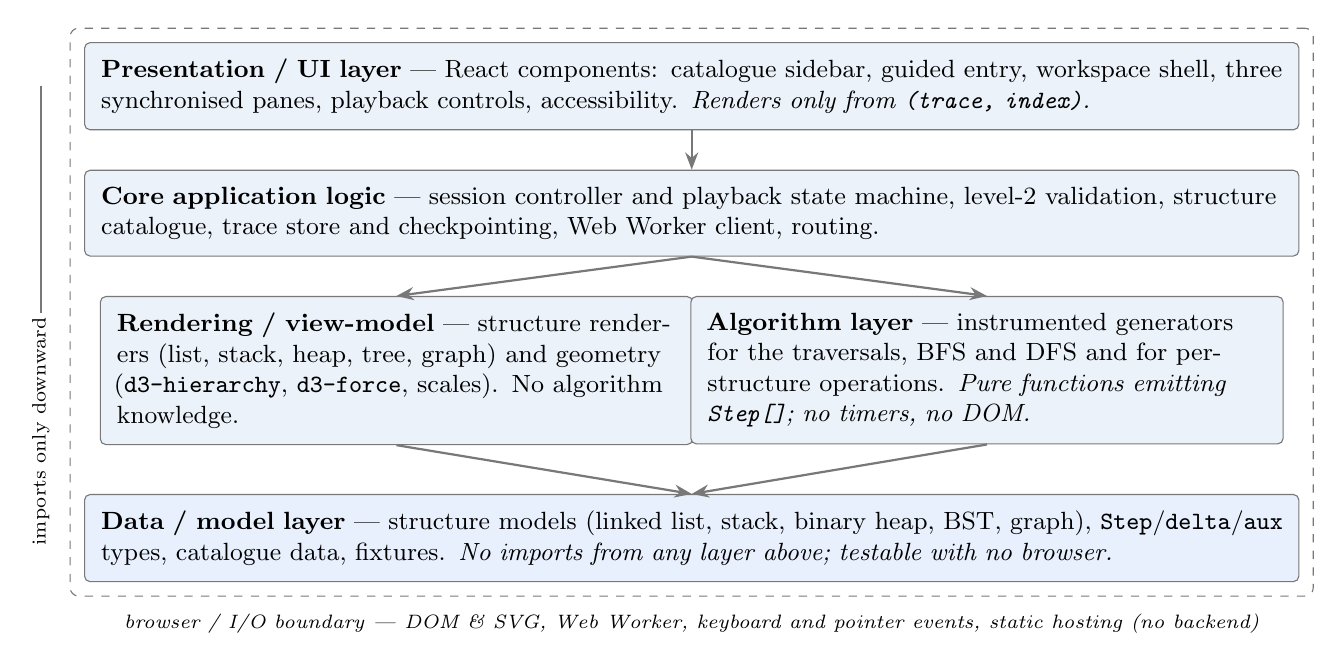
\begin{tikzpicture}
  \node[layer, text width=15cm] (l5) {\textbf{Presentation / UI layer} --- React components:
    catalogue sidebar, guided entry, workspace shell, three synchronised panes, playback
    controls, accessibility. \emph{Renders only from \ct{(trace, index)}.}};
  \node[layer, text width=15cm, below=5mm of l5] (l4) {\textbf{Core application logic} --- session
    controller and playback state machine, level-2 validation, structure catalogue, trace store
    and checkpointing, Web Worker client, routing.};
  \node[inner sep=0pt, minimum width=15cm, minimum height=0pt, below=5mm of l4] (rowanchor) {};
  \node[layer, text width=7.1cm, anchor=north, at={([xshift=-3.75cm]rowanchor.north)}] (l3)
    {\textbf{Rendering / view-model} --- structure renderers (list, stack, heap, tree, graph) and
     geometry (\ct{d3-hierarchy}, \ct{d3-force}, scales). No algorithm knowledge.};
  \node[layer, text width=7.1cm, anchor=north, at={([xshift=3.75cm]rowanchor.north)}] (l2)
    {\textbf{Algorithm layer} --- instrumented generators for the traversals, BFS and DFS and for
     per-structure operations. \emph{Pure functions emitting \ct{Step[]}; no timers, no DOM.}};
  \node[layer, text width=15cm, fill=statec, below=25mm of rowanchor] (l1)
    {\textbf{Data / model layer} --- structure models (linked list, stack, binary heap, BST,
     graph), \ct{Step}/\ct{delta}/\ct{aux} types, catalogue data, fixtures. \emph{No imports from
     any layer above; testable with no browser.}};
  \draw[e] (l5.south) -- (l4.north);
  \draw[e] (l4.south) -- (l3.north);
  \draw[e] (l4.south) -- (l2.north);
  \draw[e] (l3.south) -- (l1.north);
  \draw[e] (l2.south) -- (l1.north);
  \draw[e] ($(l5.west)+(-0.55,0)$) -- ($(l1.west)+(-0.55,0)$)
        node[lbl,left,pos=0.5,rotate=90]{imports only downward};
  \begin{scope}[on background layer]
    \node[draw=rulec, dashed, rounded corners=3pt, fit=(l5)(l1)(l3)(l2), inner sep=5pt] (bound) {};
    \node[font=\scriptsize\itshape, below=1mm of bound, align=center]
      {browser / I/O boundary --- DOM \& SVG, Web Worker, keyboard and pointer events,
       static hosting (no backend)};
  \end{scope}
\end{tikzpicture}
\caption{Layered architecture. Imports point only downwards, so the data and algorithm layers run
and are tested without a browser. The rendering and algorithm layers are siblings: both depend on
the model. Only the core knows about time; only the UI layer knows about the DOM.}
\label{fig:layers}
\end{figure}

\subsection{Component responsibilities}

\begin{table}[H]
\centering
\small
\setlength{\tabcolsep}{4pt}
\begin{tabular}{@{}L{3.0cm}L{4.8cm}L{4.3cm}L{3.1cm}@{}}
\toprule
\textbf{Component} & \textbf{Responsibility} & \textbf{Depends on} & \textbf{Must not} \\
\midrule
UI shell and panes & Catalogue, guide, three panes, controls, narration, a11y. &
Core logic, rendering, model types. & Hold a timer, mutate a step index, import the algorithm
directly. \\
Session controller & Owns the single mutable index and the single timer; state machine. &
Model types. & Know about React or the DOM. \\
Validator & Total, per-token validation before construction; produces the report. &
Model types. & Repair input silently or forward raw text. \\
Trace store & Delta log + checkpoints; \ct{reconstruct(i)}; serialisation. &
Model and trace types. & Know why a step exists. \\
Catalogue & Static \ct{OperationMeta} records that drive menu, guide, pseudocode id and complexity. &
Model types. & Fetch over the network. \\
Rendering layer & Pure \ct{(modelAtI, step)} $\to$ SVG; layout mathematics. &
Model and trace types, D3 geometry. & Read the algorithm or own the step index. \\
Algorithm generators & Pure \ct{(structure, request)} $\to$ \ct{\{trace, summary\}}. &
Model and trace types. & Import React, D3 or any renderer. \\
Structure models & Data and invariants for the five structures. & Nothing. & Know about layout or
the UI. \\
I/O adapters & Worker messages, DOM events, static hosting. & Model types. & Contain algorithm or
presentation logic. \\
\bottomrule
\end{tabular}
\caption{Component responsibilities and the dependency rule each one enforces.}
\end{table}

\subsection{Module map}

\A\ The repository layout below is the architecture made concrete: each of the six module groups of
Section~5.1 maps to one top-level directory, and the table records what each is allowed to import.
The boundary is enforced mechanically rather than by convention --- an ESLint rule rejects any
import of React, D3, \ct{render/} or \ct{ui/} from inside \ct{core/}, and the core test suite runs
in Node with no DOM.

\begin{table}[H]
\centering
\small
\setlength{\tabcolsep}{4pt}
\begin{tabular}{@{}L{2.3cm}L{3.0cm}L{6.4cm}L{3.3cm}@{}}
\toprule
\textbf{Layer} & \textbf{Directory} & \textbf{Contents} & \textbf{May import} \\
\midrule
Data / model & \ct{core/model/}, \ct{core/trace/} & The five structure models; the \ct{Step},
\ct{StructureDelta} and \ct{AuxState} types; the trace store; catalogue data; fixtures. & Nothing
outside itself; no DOM. \\
Algorithm & \ct{core/operations/} & One generator per operation --- list, stack, heap, BST, the
four traversals, BFS and DFS --- each a pure function emitting \ct{Step[]}. & Model and trace types
only. \\
Rendering & \ct{render/} & One renderer per structure, plus the geometry that feeds it
(\ct{d3-hierarchy}, \ct{d3-force}, scales). & Model and trace types; D3 geometry. \\
Core application & \ct{app/} & Session controller and playback state machine, validation, the
catalogue, the Web Worker client and worker, routing. & Model and trace types. \\
Presentation & \ct{ui/} & Shell, sidebar, guide, the three panes, playback controls,
accessibility, per-panel error boundaries. & Core logic, rendering, model types. \\
I/O adapters & \ct{app/worker*}, event handlers in \ct{ui/} & Worker message passing, DOM and
pointer events, static hosting. & Model types. \\
\bottomrule
\end{tabular}
\caption{Layer-to-directory mapping and the import rule each layer obeys. Imports may cross
boundaries only downwards, and the ESLint rule fails the build otherwise.}
\label{tab:modules}
\end{table}

\begin{lstlisting}[style=ts,caption={Proposed source layout. One module per structure, one file per
operation; the trace types live in exactly one place so generator and renderer cannot drift.},
label={lst:layout}]
src/
  core/                         # layers 1-2: no UI imports, no DOM, no timers
    model/
      linkedList.ts  stack.ts  binaryHeap.ts  bst.ts  graph.ts
    trace/
      step.ts                   # Step, StructureDelta, AuxState (the contract)
      store.ts                  # delta log + checkpoints, reconstruct(index)
    operations/
      list/   insertAtHead.ts  insertAt.ts  deleteByValue.ts  reverse.ts
      stack/  push.ts  pop.ts
      heap/   insert.ts  extractMin.ts  buildHeap.ts
      bst/    insert.ts  delete.ts  search.ts  minMax.ts
      traverse/ preorder.ts  inorder.ts  postorder.ts  levelOrder.ts
      graph/  bfs.ts  dfs.ts
  app/                          # layer 3: session + playback + I/O adapters
    controller.ts  stateMachine.ts  validate.ts  catalogue.ts
    workerClient.ts  worker.ts  routes.ts
  render/                       # layer 4: geometry only
    renderers/ list.tsx stack.tsx heap.tsx tree.tsx graph.tsx
    layout/    hierarchy.ts  force.ts  scales.ts
  ui/                           # layer 5: presentation
    shell/  sidebar/  guide/  panes/  controls/  a11y/  ErrorBoundary.tsx
  data/                         # static, versioned
    catalogue.ts  presets/*.json  golden/*.json
tests/
  core/         # pure unit + property tests, no DOM
  golden/       # trace snapshot tests
  e2e/          # one Playwright walkthrough
\end{lstlisting}

\subsection{How the components interact}

\noindent\textbf{The request pipeline.} Every operation follows the same five stages, and only
\ct{generateTrace} differs between operations. This is the pipeline Assignment~1 fixed and
Assignment~2 implements:

\begin{enumerate}[leftmargin=1.6em,topsep=2pt,itemsep=2pt]
  \item \textbf{Parse.} User text becomes candidate tokens. No side effects.
  \item \textbf{Validate.} Every token is classified against the structure's rules; the accepted
        list is the only thing that ever reaches the algorithm (FR6, ER1--ER3, ER8).
  \item \textbf{Build.} The accepted values construct the initial structure.
  \item \textbf{Execute.} The instrumented generator produces an ordered \ct{Step[]}, optionally
        in a Web Worker. This stage is pure, deterministic and DOM-free (FR7).
  \item \textbf{Present.} The controller loads the trace and sets the index to~$0$; from this point
        the interface is a pure function of \ct{(trace, index)} (FR8--FR11).
\end{enumerate}

\begin{figure}[htbp]
\centering
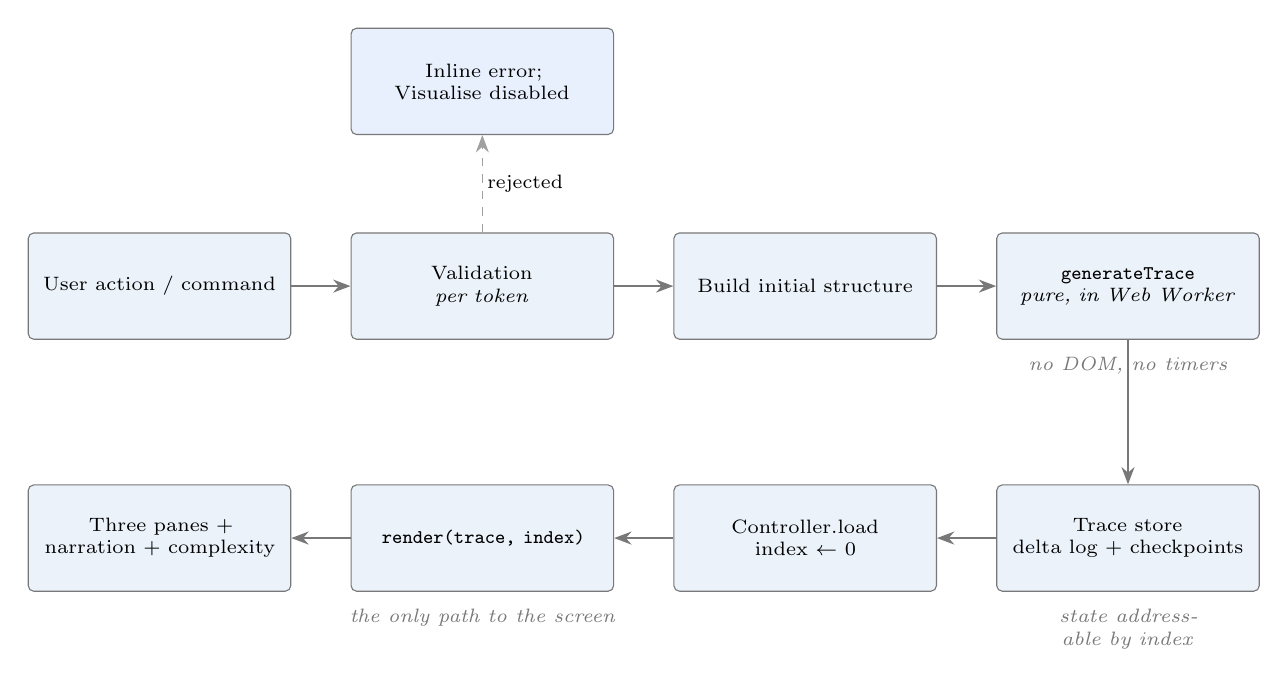
\begin{tikzpicture}[
  seq/.style={draw=rulec, rounded corners=2pt, fill=boxc, align=center,
              font=\scriptsize, text width=3.1cm, minimum height=1.35cm},
  note/.style={font=\scriptsize\itshape, color=rulec, align=center}]
  \node[seq] (a) at (0,0) {User action / command};
  \node[seq] (b) at (4.1,0) {Validation\\ \emph{per token}};
  \node[seq] (c) at (8.2,0) {Build initial structure};
  \node[seq] (d) at (12.3,0) {\ct{generateTrace}\\ \emph{pure, in Web Worker}};
  \node[seq, fill=statec] (err) at (4.1,2.6) {Inline error;\\ Visualise disabled};
  \node[seq] (e) at (12.3,-3.2) {Trace store\\ delta log + checkpoints};
  \node[seq] (f) at (8.2,-3.2) {Controller.load\\ index $\leftarrow$ 0};
  \node[seq] (g) at (4.1,-3.2) {\ct{render(trace, index)}};
  \node[seq] (h) at (0,-3.2) {Three panes +\\ narration + complexity};
  \draw[e] (a) -- (b);
  \draw[e] (b) -- (c);
  \draw[e] (c) -- (d);
  \draw[e] (d) -- (e);
  \draw[e] (e) -- (f);
  \draw[e] (f) -- (g);
  \draw[e] (g) -- (h);
  \draw[ed] (b) -- node[lbl,right]{rejected} (err);
  \node[note, below=1mm of d] {no DOM, no timers};
  \node[note, below=1mm of g] {the only path to the screen};
  \node[note, below=1mm of e, text width=2.8cm] {state addressable by index};
\end{tikzpicture}
\caption{The request pipeline. Validation is total and precedes construction; execution is pure and
optionally off the main thread; presentation is a pure function of the stored trace and a single
index.}
\label{fig:pipeline}
\end{figure}

\noindent\textbf{Steady-state playback.} Once a trace is loaded, every control is an operation on the
index. The controller advances or clamps the index, publishes it, and each pane re-renders from
\ct{trace[index]}. Because the trace is immutable and precomputed, a frame is a repaint and never an
algorithm execution, which is what makes step-back exact and rapid input harmless.

\begin{figure}[htbp]
\centering
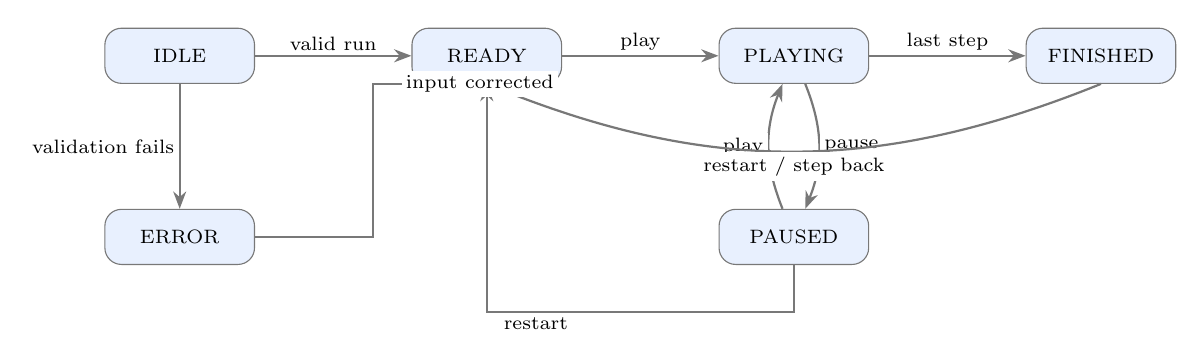
\begin{tikzpicture}[>={Stealth[length=2.2mm]},
  st/.style={draw=rulec, rounded corners=6pt, fill=statec, minimum height=7mm,
             minimum width=19mm, align=center, font=\scriptsize}]
  \node[st] (idle) at (0,0) {IDLE};
  \node[st] (ready) at (3.9,0) {READY};
  \node[st] (playing) at (7.8,0) {PLAYING};
  \node[st] (fin) at (11.7,0) {FINISHED};
  \node[st] (paused) at (7.8,-2.3) {PAUSED};
  \node[st] (err) at (0,-2.3) {ERROR};
  \draw[e] (idle) -- node[lbl,above]{valid run} (ready);
  \draw[e] (ready) -- node[lbl,above]{play} (playing);
  \draw[e] (playing) -- node[lbl,above]{last step} (fin);
  \draw[e] (playing) to[bend left=22] node[lbl,right]{pause} (paused);
  \draw[e] (paused) to[bend left=22] node[lbl,left]{play} (playing);
  \draw[e] (fin.south) to[bend left=22] node[lbl,below]{restart / step back} (ready.south);
  \draw[e] (paused.south) -- ++(0,-0.6) -| node[lbl,below,pos=0.42]{restart} (ready.south);
  \draw[e] (idle) -- node[lbl,left]{validation fails} (err);
  \draw[e] (err.east) -- ++(1.5,0) |- node[lbl,right,pos=0.62]{input corrected} (ready.south);
\end{tikzpicture}
\caption{The session state machine. \ct{PLAYING} is the only state that owns a timer; READY, PAUSED
and FINISHED all hold a valid trace, so every control is clamped index arithmetic and phase and
index cannot disagree.}
\label{fig:states}
\end{figure}

\subsection{Interfaces}

The interface between the two halves of the team --- and between the algorithm and the UI --- is
typed and frozen before the structure catalogue is expanded (Section~5.7). The central type is the
\ct{Step} record of Listing~\ref{lst:step}; the table below lists the seams.

\begin{table}[H]
\centering
\small
\setlength{\tabcolsep}{4pt}
\begin{tabular}{@{}L{3.6cm}L{11.6cm}@{}}
\toprule
\textbf{Interface} & \textbf{Contract and direction} \\
\midrule
\ct{Step}, \ct{StructureDelta}, \ct{AuxState} & Algorithm $\to$ trace store $\to$ renderer. The
frozen contract; see Listing~\ref{lst:step}. Serialisable and deterministic. \\
\ct{generate(structure, request)} & Algorithm layer. Pure; returns \ct{\{trace, summary\}}, where
the summary carries the step count, comparison count and conclusion. \\
\ct{OperationMeta} & Catalogue $\to$ menu, guide, pseudocode id, complexity card. Listing~\ref{lst:opmeta}. \\
\ct{reconstruct(i)} & Trace store $\to$ renderer. Returns the structure and \ct{aux} at index $i$
from the nearest checkpoint plus at most $k-1$ deltas. \\
\ct{CatalogueEntry} & Static data $\to$ sidebar and router. A structure's description, rules,
presets and operation list. \\
\ct{PlaybackController} & UI $\to$ core. \ct{load}, \ct{play}, \ct{pause}, \ct{stepForward},
\ct{stepBack}, \ct{restart}, \ct{seek}; each is idempotent and clamped. \\
Worker messages & Core $\to$ Web Worker. \ct{GenerateRequest} in, \ct{GenerateResponse} or
\ct{GenerateError} out; both structured-clone safe. \\
Validation report & Validator $\to$ UI. Per-token status with a reason; total, never repairing
silently. \\
\bottomrule
\end{tabular}
\caption{Interface seams and their direction. Each is typed in TypeScript strict mode in one shared
types module.}
\end{table}

\subsection{Design principles and how they are enforced}

\begin{table}[H]
\centering
\small
\setlength{\tabcolsep}{4pt}
\begin{tabular}{@{}L{4.1cm}L{5.6cm}L{5.5cm}@{}}
\toprule
\textbf{Principle} & \textbf{Mechanism} & \textbf{Failure it prevents} \\
\midrule
Algorithms independent of presentation & Downward-only imports; ESLint boundary; core tests run in
Node with no DOM. & A visualiser that cannot be tested or reused. \\
One source of truth & The interface is \ct{render(trace[index])}; only the controller writes the
index. & Panes drifting apart; stale elements on step-back. \\
One timer owner & Only \ct{PLAYING} holds a timer; play is idempotent. & Duplicate animation loops
(ER12). \\
Determinism & Fixed neighbour order; no wall-clock or randomness in generation; golden traces. &
Non-reproducible runs; impossible exact replay. \\
Purity and testability & Generators are pure functions of plain data; one shared types module. &
Generator and renderer diverging silently. \\
Failure containment & Validation before construction; per-panel React error boundaries; step budget
truncates and discloses (ER11, ER13). & One bad input or panel taking down the whole session. \\
Accessibility by construction & Keyboard commands are the same code path as buttons; every node
state carries a label or shape; \ct{prefers-reduced-motion} only affects view interpolation
(NFR-U2). & Colour-only meaning; controls unreachable on a projector or by keyboard. \\
\bottomrule
\end{tabular}
\caption{Design principles, the mechanism that enforces each, and the failure it prevents.}
\end{table}

\subsection{Extensibility and the build order}

\noindent\textbf{The acceptance test for extensibility.} \A\ Adding an operation must not require a
change to the controller, the state machine or the UI shell. It requires exactly three edits:

\begin{enumerate}[leftmargin=1.6em,topsep=2pt,itemsep=1pt]
  \item one instrumented generator in \ct{core/operations/} that emits \ct{Step[]};
  \item one authored pseudocode listing plus its \ct{codeLine} map; and
  \item one \ct{OperationMeta} catalogue record.
\end{enumerate}

\noindent A new \emph{structure} additionally needs one model module and one renderer, and nothing
else. This is the concrete meaning of the brief's requirement that the design support future
extension.

\smallskip
\noindent\textbf{Build order (one vertical slice first).} \A\ Five structures and their operations are
a large surface for two people. We therefore build one vertical slice first --- linked-list insert,
with all three panes and the controller fully working --- then freeze the \ct{Step} contract, then
add the priority queue, the BST, the traversals and the graph. After the contract is frozen, each
later operation is additive rather than invasive. This ordering is a risk control, not a
preference: the contract is the interface between the two members' work.

\subsection{Deployment and runtime view}

\A\ The application is a static bundle with no server-side computation. Trace generation for large
inputs runs in a Web Worker; the worker is terminated on reset so that no background computation
outlives a session. There is no authentication, no persistence of user data and no network call at
runtime, so the only stored artefacts are the versioned catalogue, presets and golden traces in the
repository. The production build is deployable to any static host (GitHub Pages, Netlify or Vercel),
which satisfies the portability and security requirements of Assignment~1.

\subsection{Architecture decision records}

\begin{table}[H]
\centering
\small
\setlength{\tabcolsep}{4pt}
\begin{tabular}{@{}L{1.3cm}L{4.5cm}L{9.4cm}@{}}
\toprule
\textbf{ID} & \textbf{Decision} & \textbf{Rationale and consequence} \\
\midrule
ADR-1 & The algorithm emits an immutable trace; the UI replays it. & Step-back, scrubbing, exact
replay, DOM-free testing and precomputed animation all follow from this one choice. It is the
architecture, not an optimisation. \\
ADR-2 & React renders the SVG; D3 computes geometry. & One DOM owner means no stale elements and no
transition fighting a re-render. D3 is used through submodules only (\ct{d3-hierarchy},
\ct{d3-force}, \ct{d3-scale}, \ct{d3-shape}, \ct{d3-interpolate}). \\
ADR-3 & Store a delta log with periodic checkpoints, not full snapshots. & $O(1)$ per step and
$O(k)$ display reconstruction keep the largest supported input within memory. \\
ADR-4 & One timer owner, and one mutable value (the index). & Rapid input cannot start two
animations; phase and index cannot disagree. \\
ADR-5 & The priority queue is a graded structure; the FIFO queue is a supporting structure. & The
priority queue is the mandatory structure for this iteration; FIFO queueing remains the frontier of
BFS and level-order traversal and is one catalogue entry away from promotion. \\
ADR-6 & TypeScript in strict mode, with the trace types in one module. & The trace is the interface
between two people working in parallel; types turn a silently missing panel into a compile error. \\
ADR-7 & Validation is total and precedes construction. & No malformed token ever reaches the
algorithm; the engine can assume well-typed input. \\
\bottomrule
\end{tabular}
\caption{Architecture decision records. Each is stated so that a later change is a visible reversal
rather than a silent drift.}
\end{table}

%=======================================================================
\section{Technology Stack}

\R\ The project fixes the implementation constraints: a browser application with an interactive
visualisation and step controls, no server-side computation, and a deliverable deployable as
static files. \A\ The team works in JavaScript/TypeScript in a shared repository. Within those
constraints, the stack below was chosen so that the architecture of Section~5 is enforceable
rather than aspirational: the algorithm and model layers must run with no DOM, and the trace must
cross a worker boundary and a test boundary unchanged.

\begin{table}[H]
\centering
\small
\setlength{\tabcolsep}{4pt}
\begin{tabular}{@{}L{3.0cm}L{3.6cm}L{8.4cm}@{}}
\toprule
\textbf{Component} & \textbf{Technology} & \textbf{Reason for selection} \\
\midrule
Application / UI & React 19 + Tailwind CSS + headless accessibility primitives (e.g.\ Radix) &
The application is a state machine rendered as a pure function of \ct{(trace, index)}, which is the
model React is designed for. Declarative rendering makes the labels, live regions and focus
management of NFR-U2 practical, and gives the per-panel error boundaries used by ER13. Tailwind
keeps the fixed shell and the single node-state palette local to each component; a headless
library supplies keyboard-correct menus, dialogs and tooltips. \\
Core / system components & TypeScript (strict) + Web Worker &
The core is pure, DOM-free and serialisable, so it runs in Node for tests and in a worker for large
inputs with no code change. Types make the trace contract checkable at compile time. \\
Libraries / frameworks & D3 as a computation library: \ct{d3-hierarchy}, \ct{d3-force},
\ct{d3-scale}, \ct{d3-shape}, \ct{d3-interpolate}; a tiny router for catalogue routes &
In a step-based visualiser React must own the SVG so that rendering is a pure function of the
current step. D3 is used only for geometry and layout; \ct{d3-selection} is not used for the main
visualisation. This is the single most important stack decision (ADR-2). \\
Data storage & In-memory trace store; versioned JSON for the catalogue, presets and golden traces;
\ct{localStorage} for UI preferences only &
There is no user data and no backend, so the only persisted artefacts are static and versioned in
the repository. The trace itself is session state, serialisable for the worker and for fixtures
(Section~4.8). \\
Testing & Vitest and \ct{fast-check} for the core; React Testing Library for panes; Playwright for
one end-to-end walkthrough; golden-trace snapshots; ESLint import-boundary rule &
The core is pure and DOM-free, so unit and property tests are fast and run in Node, which is also
how the architectural boundary (NFR-M2) is verified. Screenshot testing is deliberately avoided
because the visual output is expected to change often; golden traces are the stable regression
artefact. \\
Version control & Git / GitHub (Classroom repository) &
The prescribed submission channel; short-lived branches with pull-request review suit a
two-person team and keep the frozen trace contract under review. \\
Build / package tools & Vite; npm; \ct{tsc --noEmit} and ESLint in CI; GitHub Actions &
Vite gives a fast dev server with first-class TypeScript and React support, and a tree-shaken
production build that meets the payload target. CI runs type-checking, the boundary lint rule and
the core test suite on every push. \\
\bottomrule
\end{tabular}
\caption{Technology stack, mapped to the brief's component list. Each library is justified by a
design need, not by preference.}
\end{table}

\subsection{Rejected alternatives}

\A\ The brief requires the choices to be justified; a choice is only justified if the alternative
was considered. The table records the alternatives that were on the table.

\begin{table}[H]
\centering
\small
\setlength{\tabcolsep}{4pt}
\begin{tabular}{@{}L{3.4cm}L{2.9cm}L{8.7cm}@{}}
\toprule
\textbf{Concern} & \textbf{Chosen} & \textbf{Rejected alternative and why} \\
\midrule
Rendering medium & SVG (DOM) & \emph{Canvas}: faster at very large node counts, but no per-node
DOM for labels, focus and ARIA, and the graded output is at $n\le 200$, where SVG is sufficient. \\
State management & One reducer / small store for the index & \emph{Redux or a large store}: there is
exactly one mutable value plus the loaded trace; a heavy store adds indirection without buying
anything at this size, and risks putting algorithm state in the UI store. \\
DOM ownership & React owns the SVG & \emph{D3 owns the DOM}: gives two sources of truth,
transitions fighting re-renders, and stale elements when stepping backwards --- unacceptable when
the animation is the graded output. \\
Language & TypeScript strict & \emph{Plain JavaScript}: workable, but trades a one-time cost for a
class of runtime bug that is hard to debug in animation code, and the trace is the interface
between two people. \\
Test runner & Vitest & \emph{Jest}: requires extra configuration for the Vite/ESM pipeline;
Vitest reuses the build configuration and runs the DOM-free core in Node directly. \\
End-to-end & Playwright & \emph{Cypress}: both are adequate; Playwright's multi-browser support and
one-walkthrough scope fit better. Only one end-to-end path is tested, deliberately. \\
Styling & Tailwind with design tokens & \emph{Ad-hoc CSS or a full component library}: the state
palette (undiscovered / frontier / current / visited) must be defined once so colour is never the
sole signal and never chosen per component. \\
Execution thread & Main thread below threshold, Web Worker above & \emph{Always main thread}:
large inputs would block the UI and break the responsiveness target (NFR-P4). \\
Backend & None (static) & \emph{Firebase or any hosted store}: there are no accounts and no shared
state, so a backend would add failure modes, cost and a privacy surface for no benefit. \\
\bottomrule
\end{tabular}
\caption{Rejected alternatives.}
\end{table}

\subsection{Risks in the chosen stack, and mitigations}

\begin{itemize}[leftmargin=1.4em,topsep=2pt,itemsep=2pt]
  \item \textbf{Two rendering paradigms.} Mixing D3's DOM manipulation with React's rendering is
        the main technical risk. \emph{Mitigation:} the ADR-2 rule is absolute for the main
        visualisation; D3 may own the DOM only inside isolated imperative leaves such as an axis,
        which never contain React children.
  \item \textbf{Transition conflicts.} An animation library that mutates attributes React also
        renders will flicker. \emph{Mitigation:} motion is expressed as CSS transitions on
        transform and opacity, or computed by \ct{d3-interpolate} and passed to React as values,
        never applied to the DOM directly; \ct{prefers-reduced-motion} removes it entirely.
  \item \textbf{Timing drift.} \emph{Mitigation:} a single timer owner drives the index from
        elapsed time rather than counting ticks, so a slow frame drops steps instead of changing
        the logical rate (Section~5.6).
  \item \textbf{Scope size.} Five structures and their operations are a large surface for two
        people. \emph{Mitigation:} build the vertical slice first, freeze the \ct{Step} contract,
        then add structures, because extensibility is an acceptance criterion (Section~5.7).
  \item \textbf{Content drift between prose and code.} \emph{Mitigation:} the pseudocode listing,
        its line map and the complexity card all derive from one \ct{OperationMeta} record, so a
        missing or mismatched bound is a visible content gap rather than a silent omission.
\end{itemize}

\end{document}
